\section*{Глава 2. Проектирование веб-приложения}
\addcontentsline{toc}{section}{Глава 2. Проектирование веб-приложения}
\stepcounter{section}

\subsection{Анализ целевой аудитории}

Разрабатываемое приложение ориентировано на три категории пользователей фитнес-центра.
Для каждой роли составлен профиль целевого пользователя (Persona) с описанием
потребностей и ожидаемого взаимодействия с системой.

\textbf{Клиент} --- физическое лицо, посещающее фитнес-центр. Основные потребности:
просматривать актуальное расписание тренировок, записываться на занятия онлайн без
необходимости звонить администратору, отслеживать историю своих записей и управлять
профилем. Ключевые требования к интерфейсу: простота, быстрый доступ к расписанию,
возможность отмены записи.

\textbf{Тренер} --- сотрудник фитнес-центра, проводящий тренировки. Основные
потребности: управлять собственным расписанием, просматривать список записавшихся
клиентов, добавлять и редактировать тренировки, загружать фото тренировок.
Требования к интерфейсу: удобный CRUD-интерфейс, наглядное отображение
загруженности тренировок.

\textbf{Администратор} --- сотрудник, управляющий работой всей платформы.
Основные потребности: управлять пользователями и их ролями, просматривать
статистику посещаемости, контролировать расписание всех тренеров. Требования
к интерфейсу: панель с агрегированными данными, полный доступ к CRUD-операциям.

Таким образом, функциональность приложения определяется совокупностью потребностей
трёх ролей, что обусловливает необходимость разграничения прав доступа и разработки
отдельных интерфейсов для каждой роли.

\subsection{Описание функциональности приложения}

Функциональные возможности системы определяются через взаимодействие пользователей
с системой. Основные бизнес-кейсы представлены в виде \textit{User Story}:

\begin{itemize}
    \item «Я, как \textbf{клиент}, хочу просмотреть расписание тренировок и
          записаться на удобное занятие онлайн, чтобы не звонить в фитнес-центр»;
    \item «Я, как \textbf{клиент}, хочу видеть историю своих записей и иметь
          возможность отменить запись, чтобы управлять своим расписанием»;
    \item «Я, как \textbf{тренер}, хочу добавлять тренировки и видеть список
          записавшихся клиентов, чтобы планировать рабочий день»;
    \item «Я, как \textbf{администратор}, хочу управлять пользователями и
          просматривать статистику посещаемости, чтобы оптимизировать работу центра».
\end{itemize}

На рисунке~\ref{fig:use_case} представлена диаграмма вариантов использования
(Use Case), отражающая взаимодействие каждой роли с функциями системы.

\begin{figure}[ht!]
    \centering
    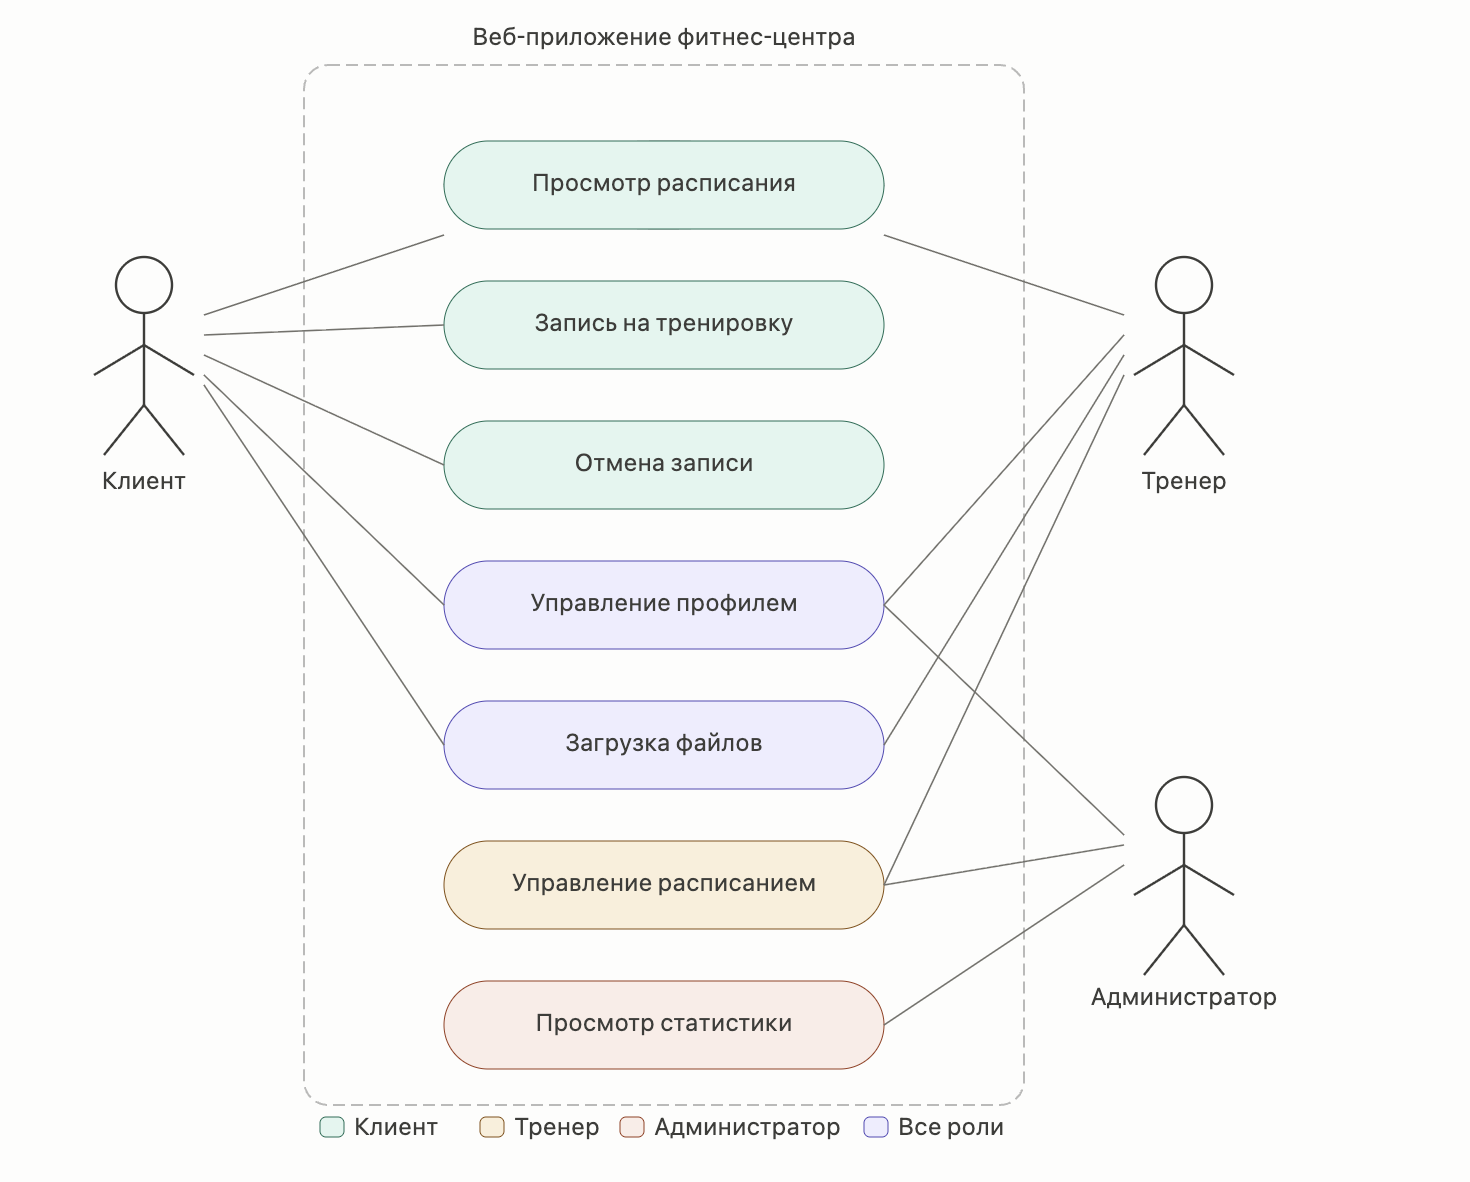
\includegraphics[width=0.85\textwidth]{images/use_case_diagram}
    \caption{Диаграмма вариантов использования системы}
    \label{fig:use_case}
\end{figure}

\subsection{Проектирование модели данных}

Модель данных приложения включает три основные сущности: пользователи
(\texttt{users}), тренировки (\texttt{workouts}) и записи на тренировки
(\texttt{bookings}). Для хранения данных используется СУБД
PostgreSQL~\cite{postgresql_docs} как наиболее подходящая реляционная система
с развитыми средствами агрегации и полной поддержкой транзакций.
Взаимодействие с базой данных реализовано через ORM-библиотеку
GORM~\cite{gorm_docs}, упрощающую написание запросов на языке Go.
ER-диаграмма базы данных представлена на рисунке~\ref{fig:er_diagram}.

\begin{figure}[ht!]
    \centering
    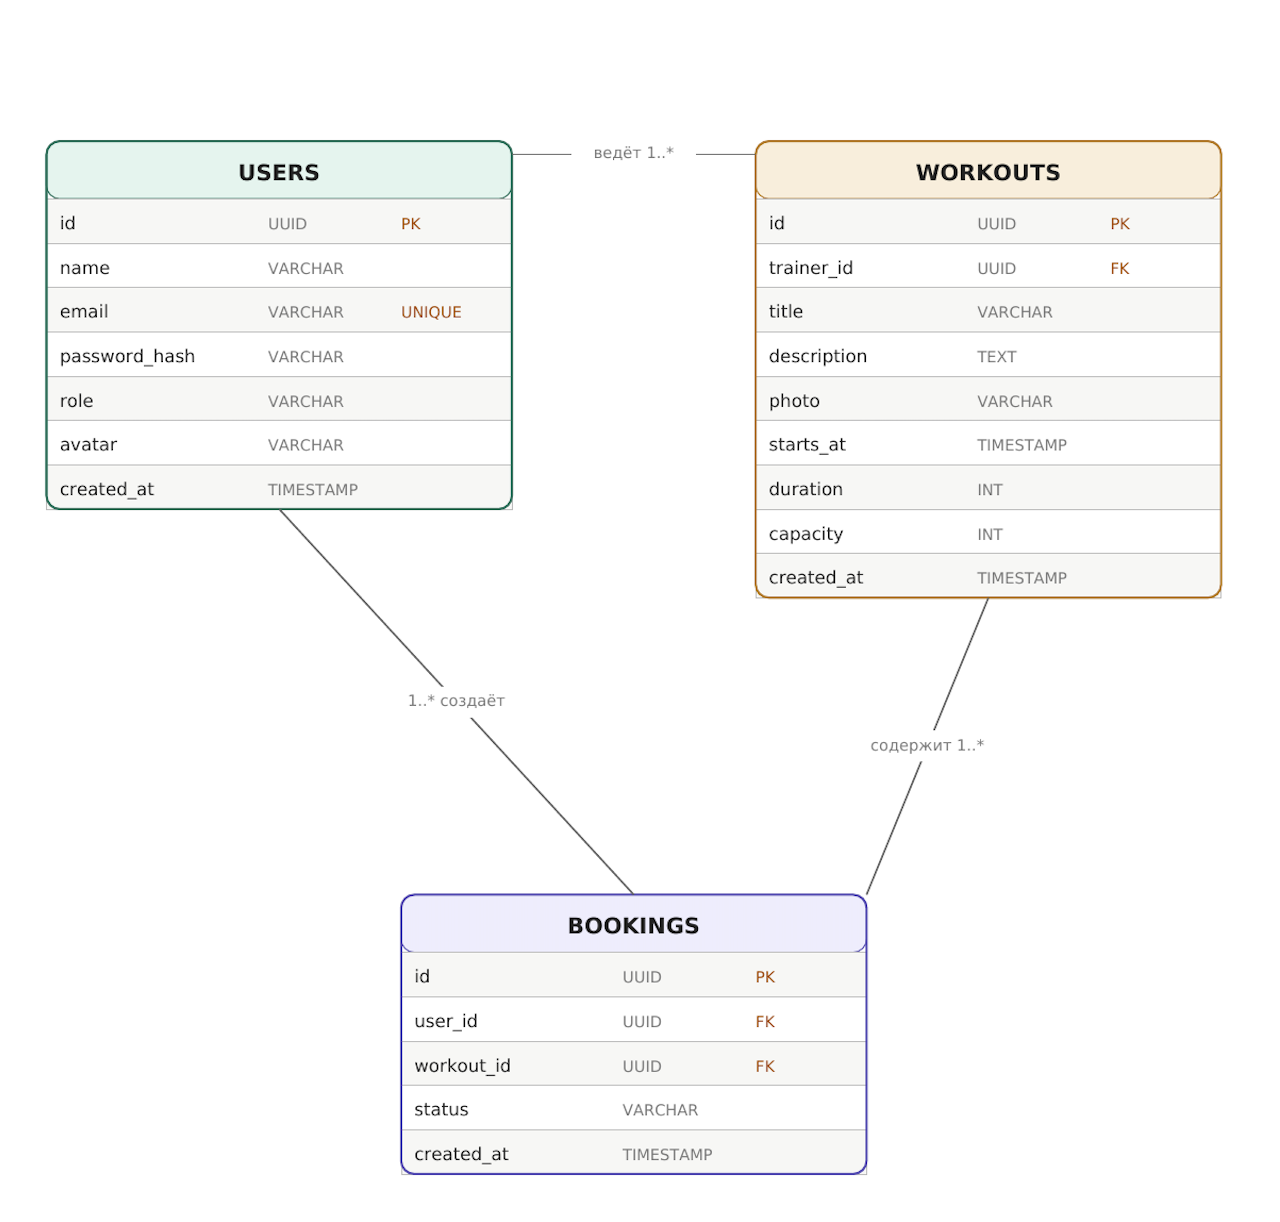
\includegraphics[width=0.85\textwidth]{images/er_diagram}
    \caption{ER-диаграмма базы данных}
    \label{fig:er_diagram}
\end{figure}

Структура таблицы пользователей представлена в табл.~\ref{tab:db_users}.

\begin{longtable}{|l|l|p{3.5cm}|p{5.5cm}|}
    \caption{Структура таблицы пользователей (\texttt{users})} \label{tab:db_users} \\

    \hline
    \textbf{Поле} & \textbf{Тип} & \textbf{Ограничение} & \textbf{Описание} \\ \hline
    \endfirsthead

    \tabcont{\ref{tab:db_users}}
    \textbf{Поле} & \textbf{Тип} & \textbf{Ограничение} & \textbf{Описание} \\ \hline
    \endhead

    \hline
    \endfoot

    \hline
    \endlastfoot

    id             & UUID      & PRIMARY KEY      & Уникальный идентификатор пользователя \\ \hline
    name           & VARCHAR   & NOT NULL         & Имя пользователя                      \\ \hline
    email          & VARCHAR   & UNIQUE, NOT NULL & Электронная почта                     \\ \hline
    password\_hash & VARCHAR   & NOT NULL         & Хэш пароля                            \\ \hline
    role           & VARCHAR   & NOT NULL         & Роль: client, trainer, admin          \\ \hline
    avatar         & VARCHAR   & NULL             & Путь к файлу аватара                  \\ \hline
    created\_at    & TIMESTAMP & DEFAULT NOW()    & Дата регистрации                      \\ \hline
\end{longtable}

Структура таблицы тренировок представлена в табл.~\ref{tab:db_workouts}.

\begin{longtable}{|l|l|p{3.5cm}|p{5.5cm}|}
    \caption{Структура таблицы тренировок (\texttt{workouts})} \label{tab:db_workouts} \\

    \hline
    \textbf{Поле} & \textbf{Тип} & \textbf{Ограничение} & \textbf{Описание} \\ \hline
    \endfirsthead

    \tabcont{\ref{tab:db_workouts}}
    \textbf{Поле} & \textbf{Тип} & \textbf{Ограничение} & \textbf{Описание} \\ \hline
    \endhead

    \hline
    \endfoot

    \hline
    \endlastfoot

    id          & UUID      & PRIMARY KEY   & Уникальный идентификатор тренировки   \\ \hline
    trainer\_id & UUID      & FOREIGN KEY   & Ссылка на таблицу пользователей       \\ \hline
    title       & VARCHAR   & NOT NULL      & Название тренировки                   \\ \hline
    description & TEXT      & NULL          & Описание тренировки                   \\ \hline
    photo       & VARCHAR   & NULL          & Путь к фото тренировки                \\ \hline
    starts\_at  & TIMESTAMP & NOT NULL      & Дата и время начала                   \\ \hline
    duration    & INT       & NOT NULL      & Длительность, минут                   \\ \hline
    capacity    & INT       & NOT NULL      & Максимальное число участников         \\ \hline
    created\_at & TIMESTAMP & DEFAULT NOW() & Время создания записи                 \\ \hline
\end{longtable}

Структура таблицы записей на тренировки представлена в табл.~\ref{tab:db_bookings}.

\begin{longtable}{|l|l|p{3.5cm}|p{5.5cm}|}
    \caption{Структура таблицы записей (\texttt{bookings})} \label{tab:db_bookings} \\

    \hline
    \textbf{Поле} & \textbf{Тип} & \textbf{Ограничение} & \textbf{Описание} \\ \hline
    \endfirsthead

    \tabcont{\ref{tab:db_bookings}}
    \textbf{Поле} & \textbf{Тип} & \textbf{Ограничение} & \textbf{Описание} \\ \hline
    \endhead

    \hline
    \endfoot

    \hline
    \endlastfoot

    id          & UUID      & PRIMARY KEY      & Уникальный идентификатор записи       \\ \hline
    user\_id    & UUID      & FOREIGN KEY      & Ссылка на таблицу пользователей       \\ \hline
    workout\_id & UUID      & FOREIGN KEY      & Ссылка на таблицу тренировок          \\ \hline
    status      & VARCHAR   & DEFAULT 'active' & Статус: active, cancelled             \\ \hline
    created\_at & TIMESTAMP & DEFAULT NOW()    & Время создания записи                 \\ \hline
\end{longtable}
\clearpage
\subsection{Разработка макетов страниц}

На этапе проектирования были разработаны макеты (Wireframe) ключевых страниц приложения, отражающие общую структуру интерфейса для каждой роли пользователя. Макеты охватывают все основные сценарии взаимодействия: просмотр расписания, аутентификацию, работу в личном кабинете клиента, управление тренировками тренером и администрирование платформы.

Макет страницы расписания (рисунок~\ref{fig:wf_schedule}) представляет главную публичную страницу приложения, доступную без авторизации. В верхней части расположена навигационная панель с логотипом, ссылками на разделы сайта и кнопками входа и регистрации. Основная область содержит фильтр по дате и тренеру, а также карточки тренировок с фотографией, названием, временем проведения, именем тренера и текущим количеством свободных мест. Каждая карточка содержит кнопку записи, доступную авторизованному клиенту.

\begin{figure}[H]
    \centering
    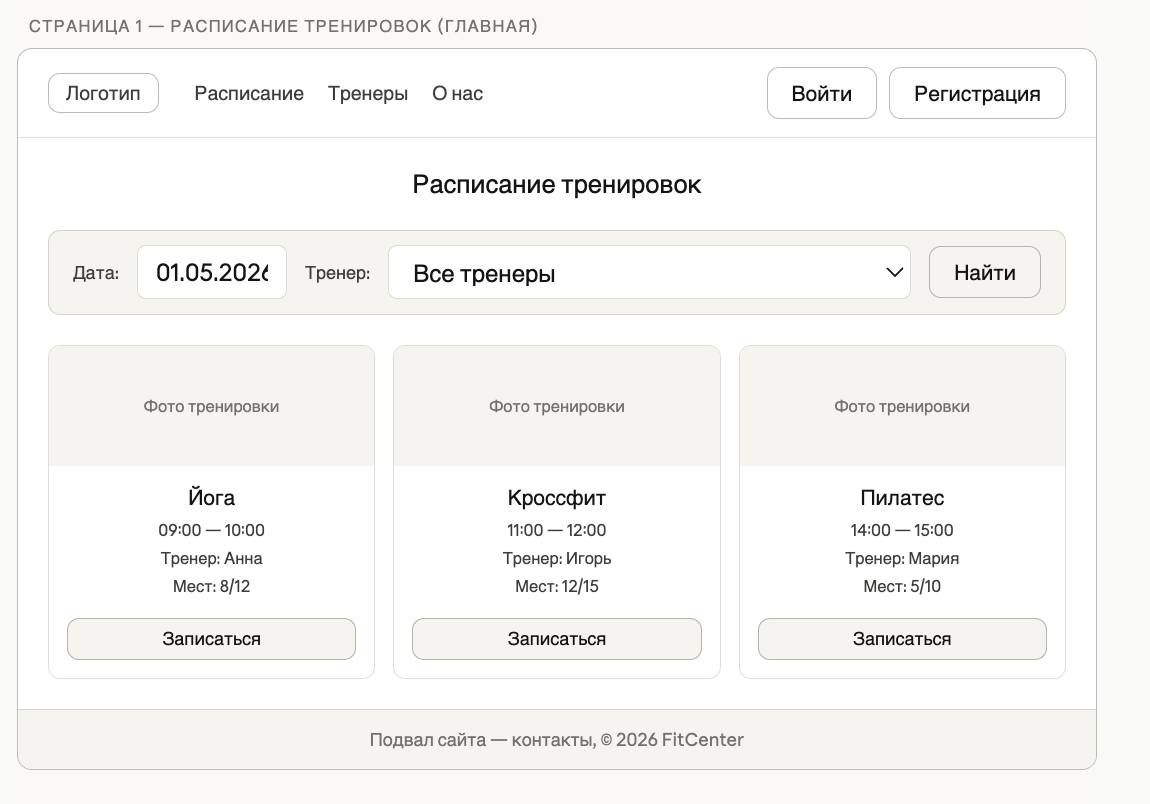
\includegraphics[width=0.75\textwidth]{images/wireframe_schedule}
    \caption{Макет страницы расписания тренировок}
    \label{fig:wf_schedule}
\end{figure}
\clearpage
Макет страницы входа (рисунок~\ref{fig:wf_login}) реализует форму аутентификации, центрированную на странице. Форма содержит поля ввода email и пароля, кнопку подтверждения, ссылку на восстановление пароля и переход к странице регистрации. В верхней части страницы расположен переключатель между вкладками «Войти» и «Регистрация», обеспечивающий навигацию между двумя формами аутентификации.

\begin{figure}[H]
    \centering
    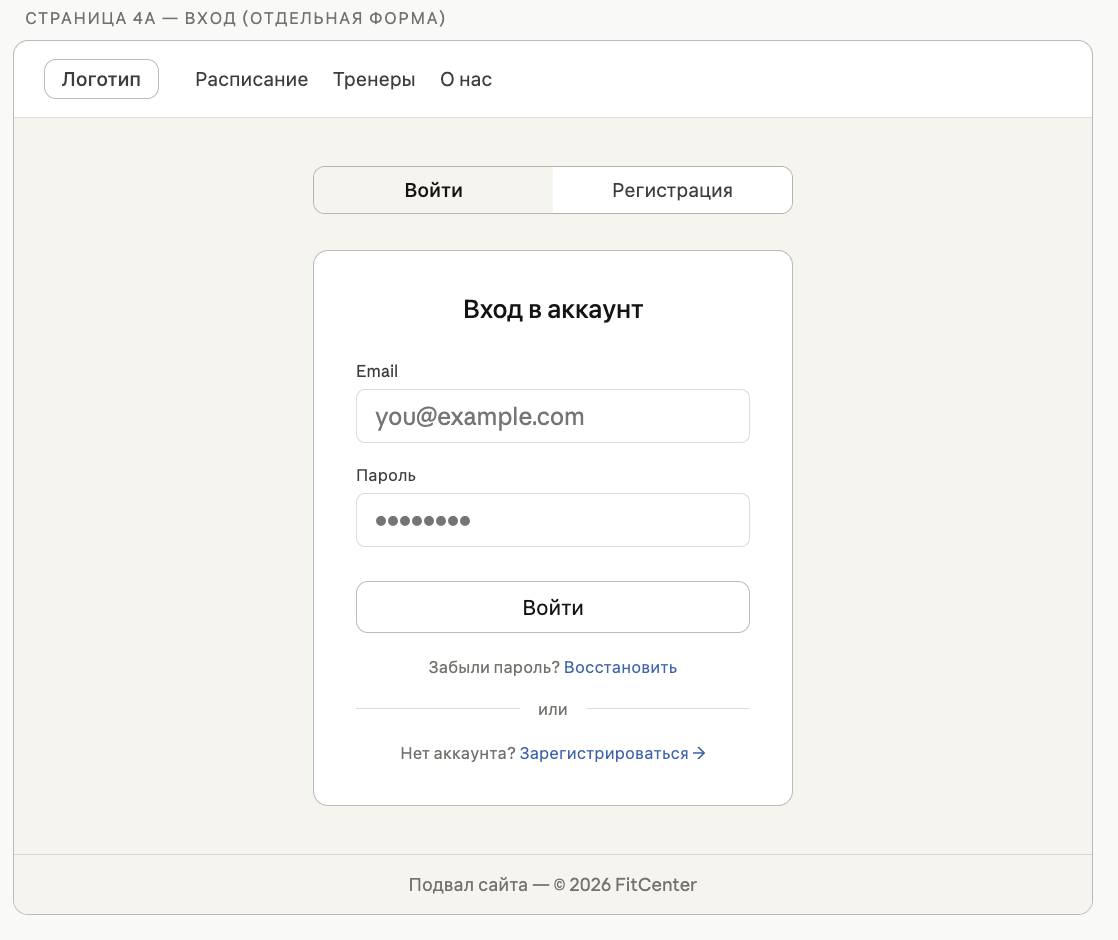
\includegraphics[width=0.75\textwidth]{images/wireframe_login}
    \caption{Макет страницы входа в аккаунт}
    \label{fig:wf_login}
\end{figure}
\clearpage
Макет страницы регистрации (рисунок~\ref{fig:wf_register}) содержит форму создания нового аккаунта с полями имени, фамилии, email, пароля, подтверждения пароля и выбора роли (клиент или тренер). Форма также центрирована на странице и использует тот же переключатель вкладок, что и страница входа, что обеспечивает единообразие интерфейса аутентификации.

\begin{figure}[H]
    \centering
    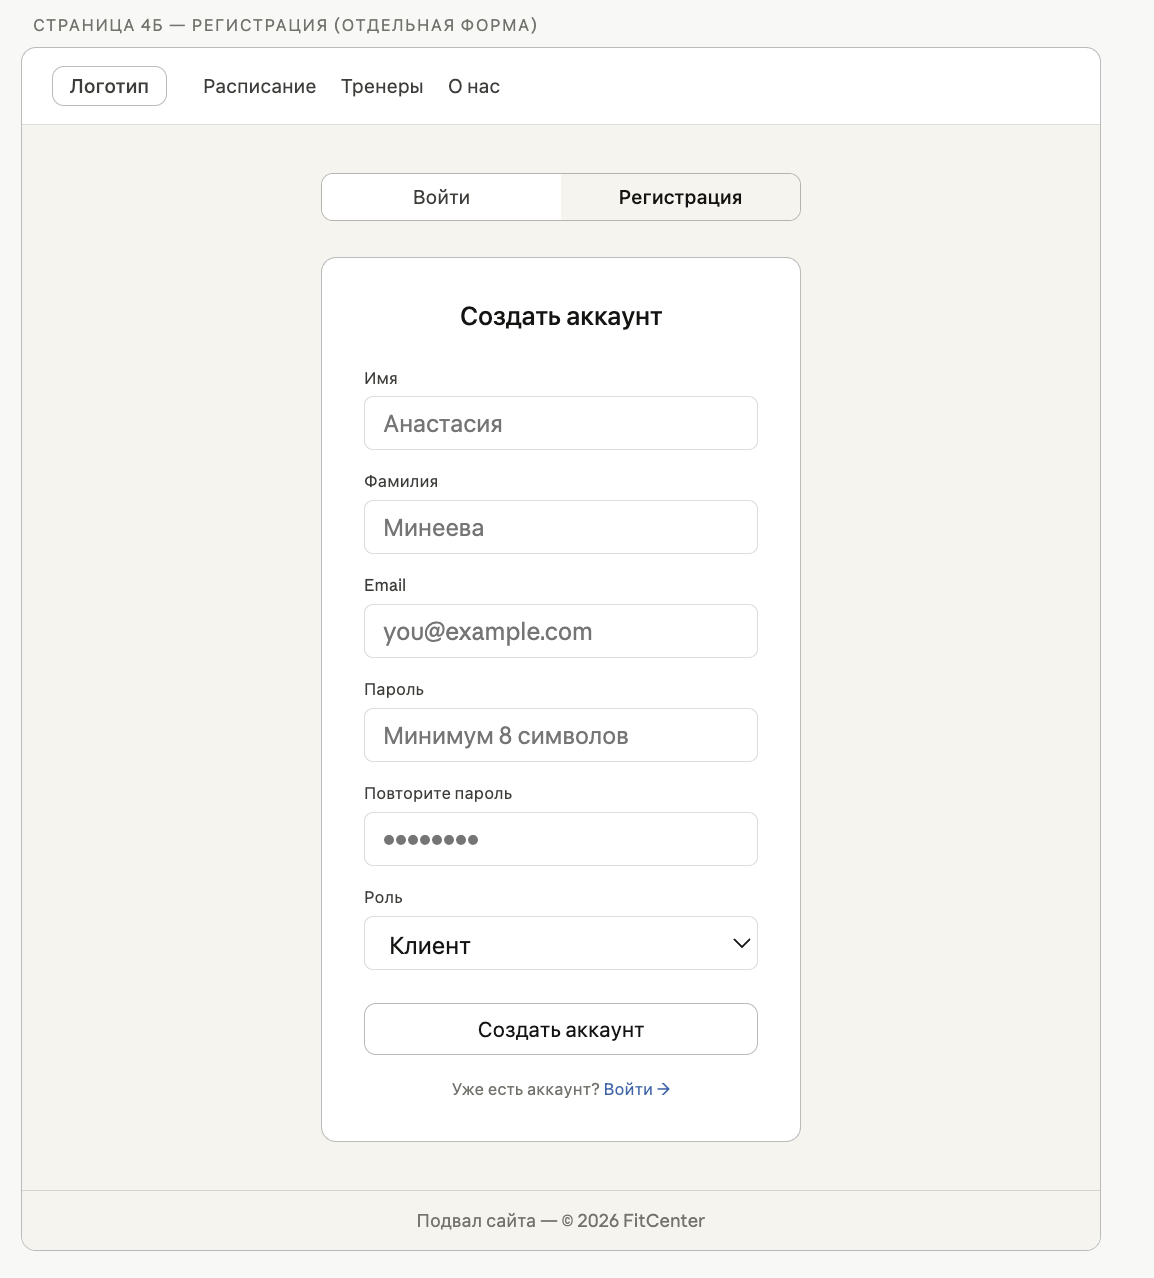
\includegraphics[width=0.75\textwidth]{images/wireframe_register}
    \caption{Макет страницы регистрации}
    \label{fig:wf_register}
\end{figure}
\clearpage
Макет личного кабинета клиента (рисунок~\ref{fig:wf_client}) разделён на боковую панель и основную рабочую область. В боковой панели отображаются аватар, имя и роль пользователя, а также кнопки навигации: смена фото, мои записи, настройки и выход. Основная область включает сводку статистики (всего записей, предстоящих и посещённых), список активных и прошедших записей с возможностью отмены, а также форму редактирования профиля с полями имени, фамилии, email и телефона.

\begin{figure}[H]
    \centering
    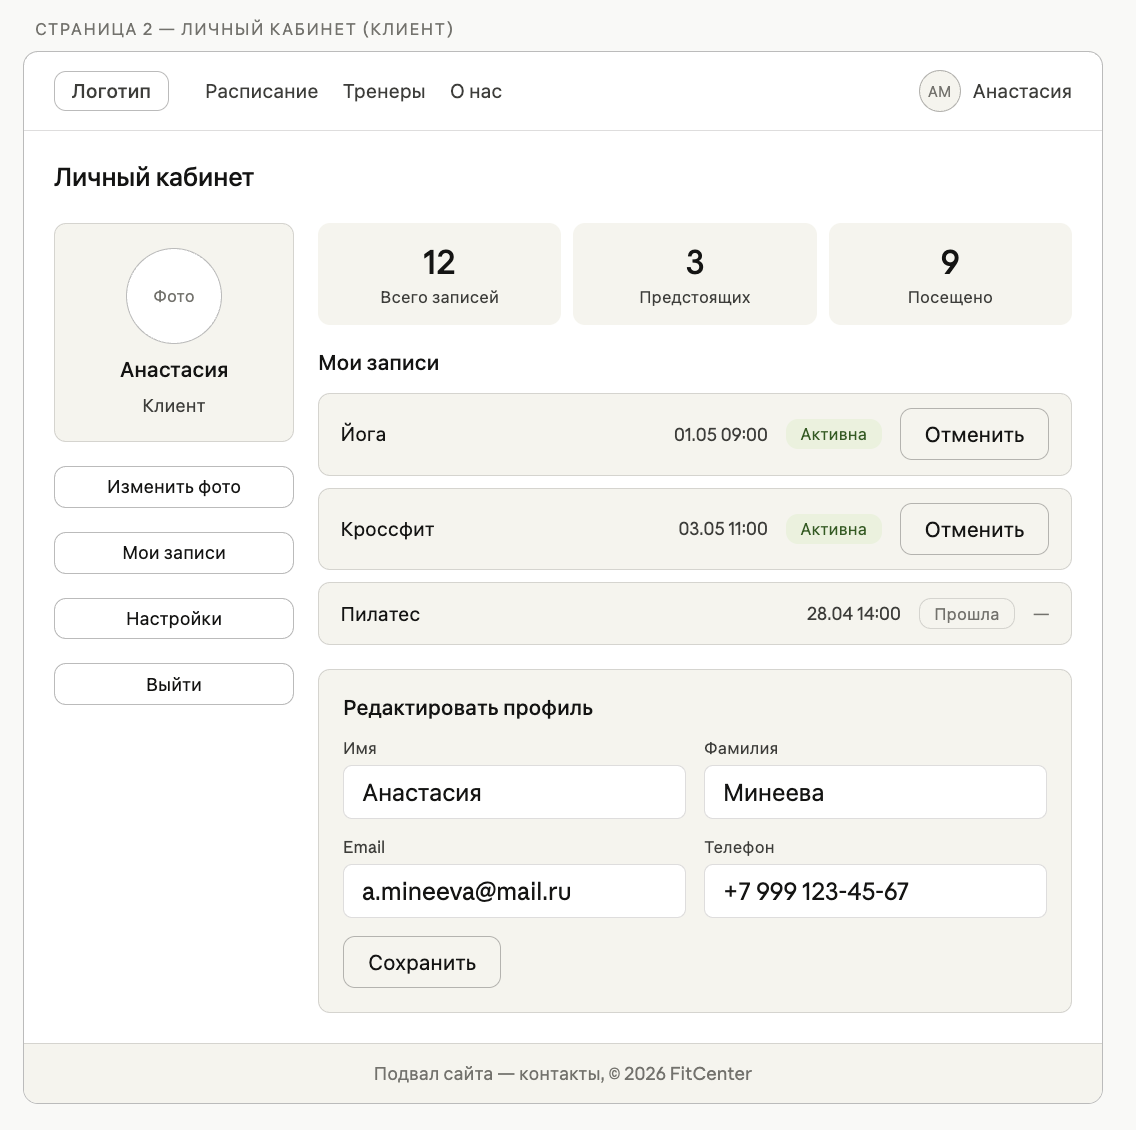
\includegraphics[width=0.75\textwidth]{images/wireframe_client}
    \caption{Макет личного кабинета клиента}
    \label{fig:wf_client}
\end{figure}
\clearpage
Макет кабинета тренера (рисунок~\ref{fig:wf_trainer}) предоставляет интерфейс управления тренировками. Боковая панель содержит навигацию по разделам кабинета: мои тренировки, мои клиенты, и профиль. В основной области отображается список тренировок тренера с указанием даты, времени, заполненности (занятых и общего числа мест) и статуса. Для каждой тренировки доступны кнопки редактирования и удаления. Ниже расположена форма добавления новой тренировки с полями названия, даты и времени, длительности, вместимости, загрузки фотографии и описания.

\begin{figure}[H]
    \centering
    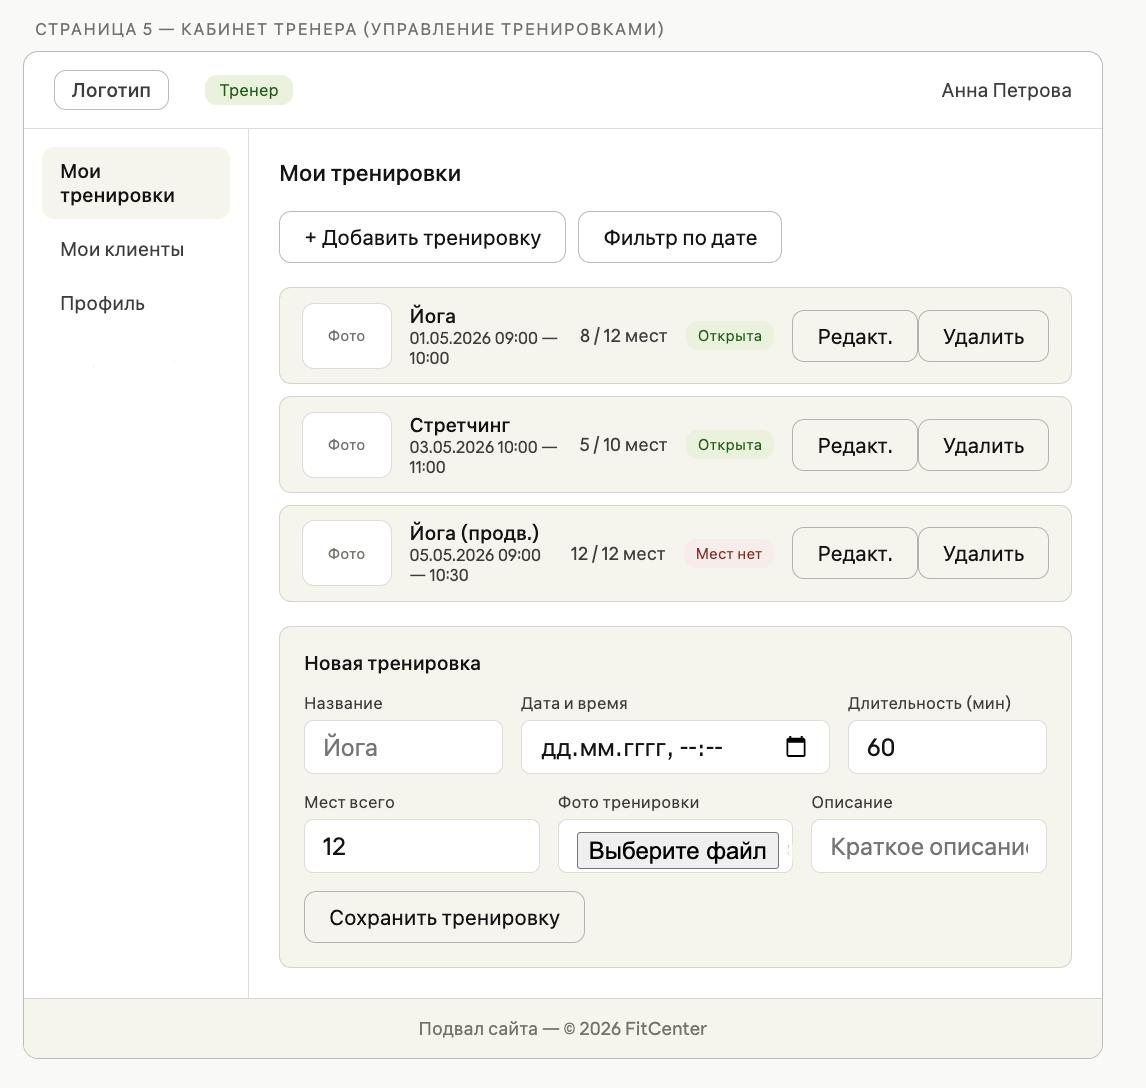
\includegraphics[width=0.75\textwidth]{images/wireframe_trainer}
    \caption{Макет кабинета тренера}
    \label{fig:wf_trainer}
\end{figure}
\clearpage
Макет панели администратора (рисунок~\ref{fig:wf_admin}) включает боковое меню с разделами: дашборд, тренировки, пользователи, расписание и статистика. На дашборде отображаются агрегированные показатели платформы: общее число записей, тренировок, тренеров и клиентов. В разделе управления пользователями представлена таблица со списком всех зарегистрированных пользователей, их email, ролью и датой регистрации. Администратор может добавлять новых пользователей, изменять их роли и удалять учётные записи.

\begin{figure}[H]
    \centering
    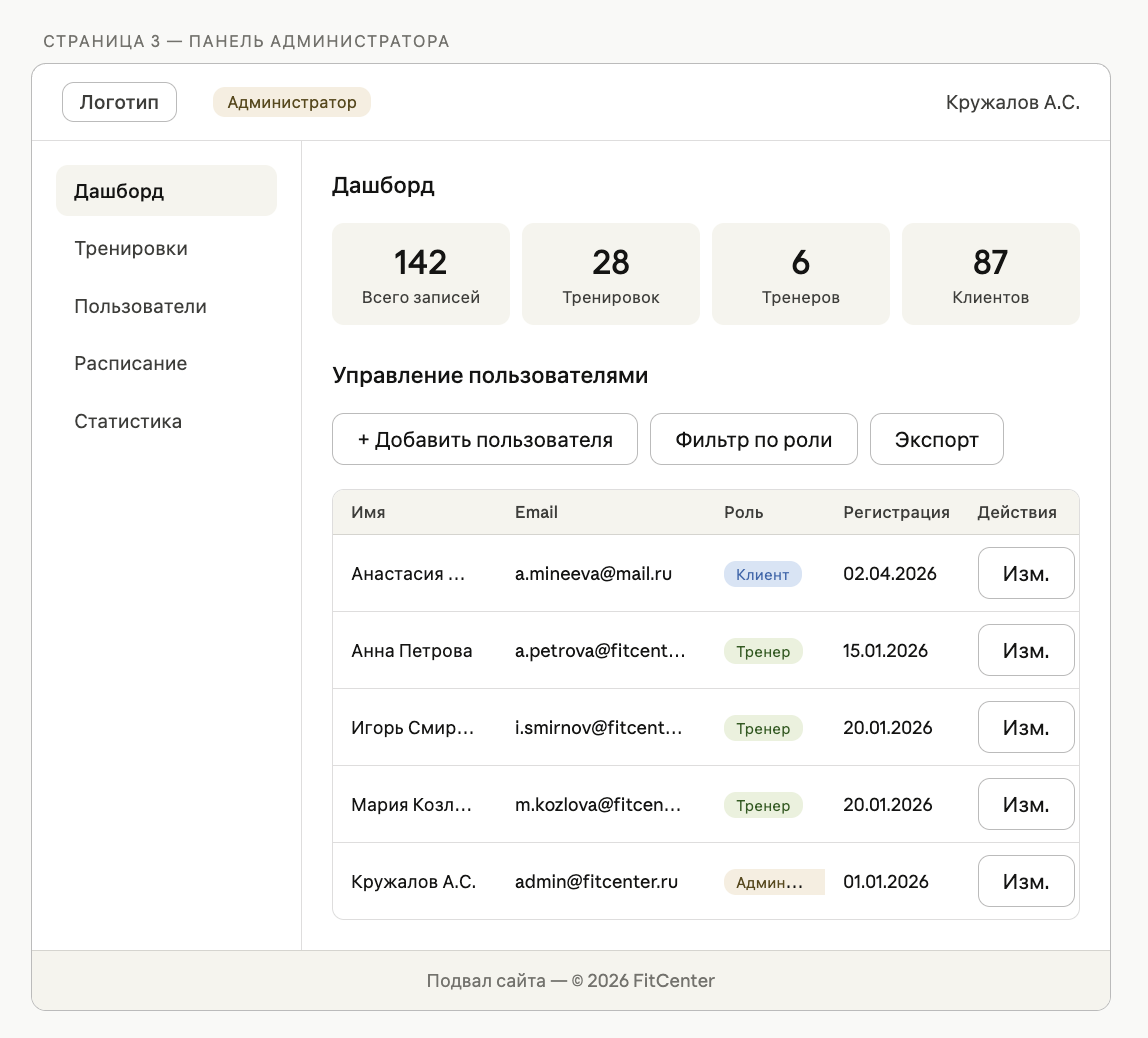
\includegraphics[width=0.75\textwidth]{images/wireframe_admin}
    \caption{Макет панели администратора}
    \label{fig:wf_admin}
\end{figure}